\chapter{Preliminary}

\section{Transformers}

Methodologies like Recurrent Neural Networks, Long Short-Term Memory, and Gated Recurrent Neural Networks have solidified their position as cutting-edge techniques in the field of sequence modeling and transduction challenges. Particularly in the areas of language modeling and machine translation is this apparent. Through several experiments, researchers have consistently pushed the limits of encoder-decoder structures and recurrent language models.


The symbolic positions of input and output sequences have traditionally been used as the foundation for recurrent models' calculations. These models create a series of hidden states denoted as $h_t$ that are influenced by the input at location t and the preceding hidden state $h_{t-1}$ by mapping these positions to computational time steps. Due to their innately sequential character, they are difficult to parallelize during training, particularly when dealing with longer sequences when memory constraints prevent batching across cases.

However, efforts have been made to increase computing efficiency using strategies such as conditional computation and factorization tricks. In some instances, the model performance has improved as a result of these developments. However, sequential computation continues to present a fundamental issue.


In an endeavor to minimize sequential computation, numerous theoretical frameworks have been developed, including the Extended Neural GPU, ByteNet, and ConvS2S. These frameworks share a common foundation centered around CNNs. Such models can compute hidden representations over all output and input places in simultaneously. Within these models, the computational complexity for establishing connections between any two arbitrary input or output locations follows a linear scaling pattern for ConvS2S and a logarithmic scaling pattern for ByteNet. The specific scaling behavior is determined by the distance between the respective positions being considered. When determining dependencies between distant sites, this scaling provides a more challenging task. The Transformer model, on the other hand, simplifies this scaling to a fixed set of actions. Despite the drawback of a reduced effective resolution caused by the averaging of attention-weighted positions, the utilization of Multi-Head Attention is employed as a countermeasure.

The Transformer model holds a unique distinction as the pioneering transduction model that exclusively employs self-attention methods to perform computations on its output and input representations, doing away with the requirement for sequence-aligned RNNs or convolutions. The Transformer model will be thoroughly described, the rationale for self-attention will be explained, and its comparative advantages over other models will be covered in the parts that follow.


\subsection{Model Architecture}
Modern neural designs for sequence transduction typically use encoder-decoder architectures. Within this particular configuration, the encoder is responsible for mapping a sequence of continuous representations, denoted as $(z_1,..., z_n)$, into a sequence of symbol representations, represented as $(x_1,..., x_n)$. Subsequently, the decoder generates an output sequence, $(y_1,..., y_m)$, iteratively, utilizing the information derived from these continuous representations. The model operates in an auto-regressive manner, incorporating the output of preceding symbols as additional input to generate the subsequent symbol at each step.

\begin{figure}[!h]
    \centering
    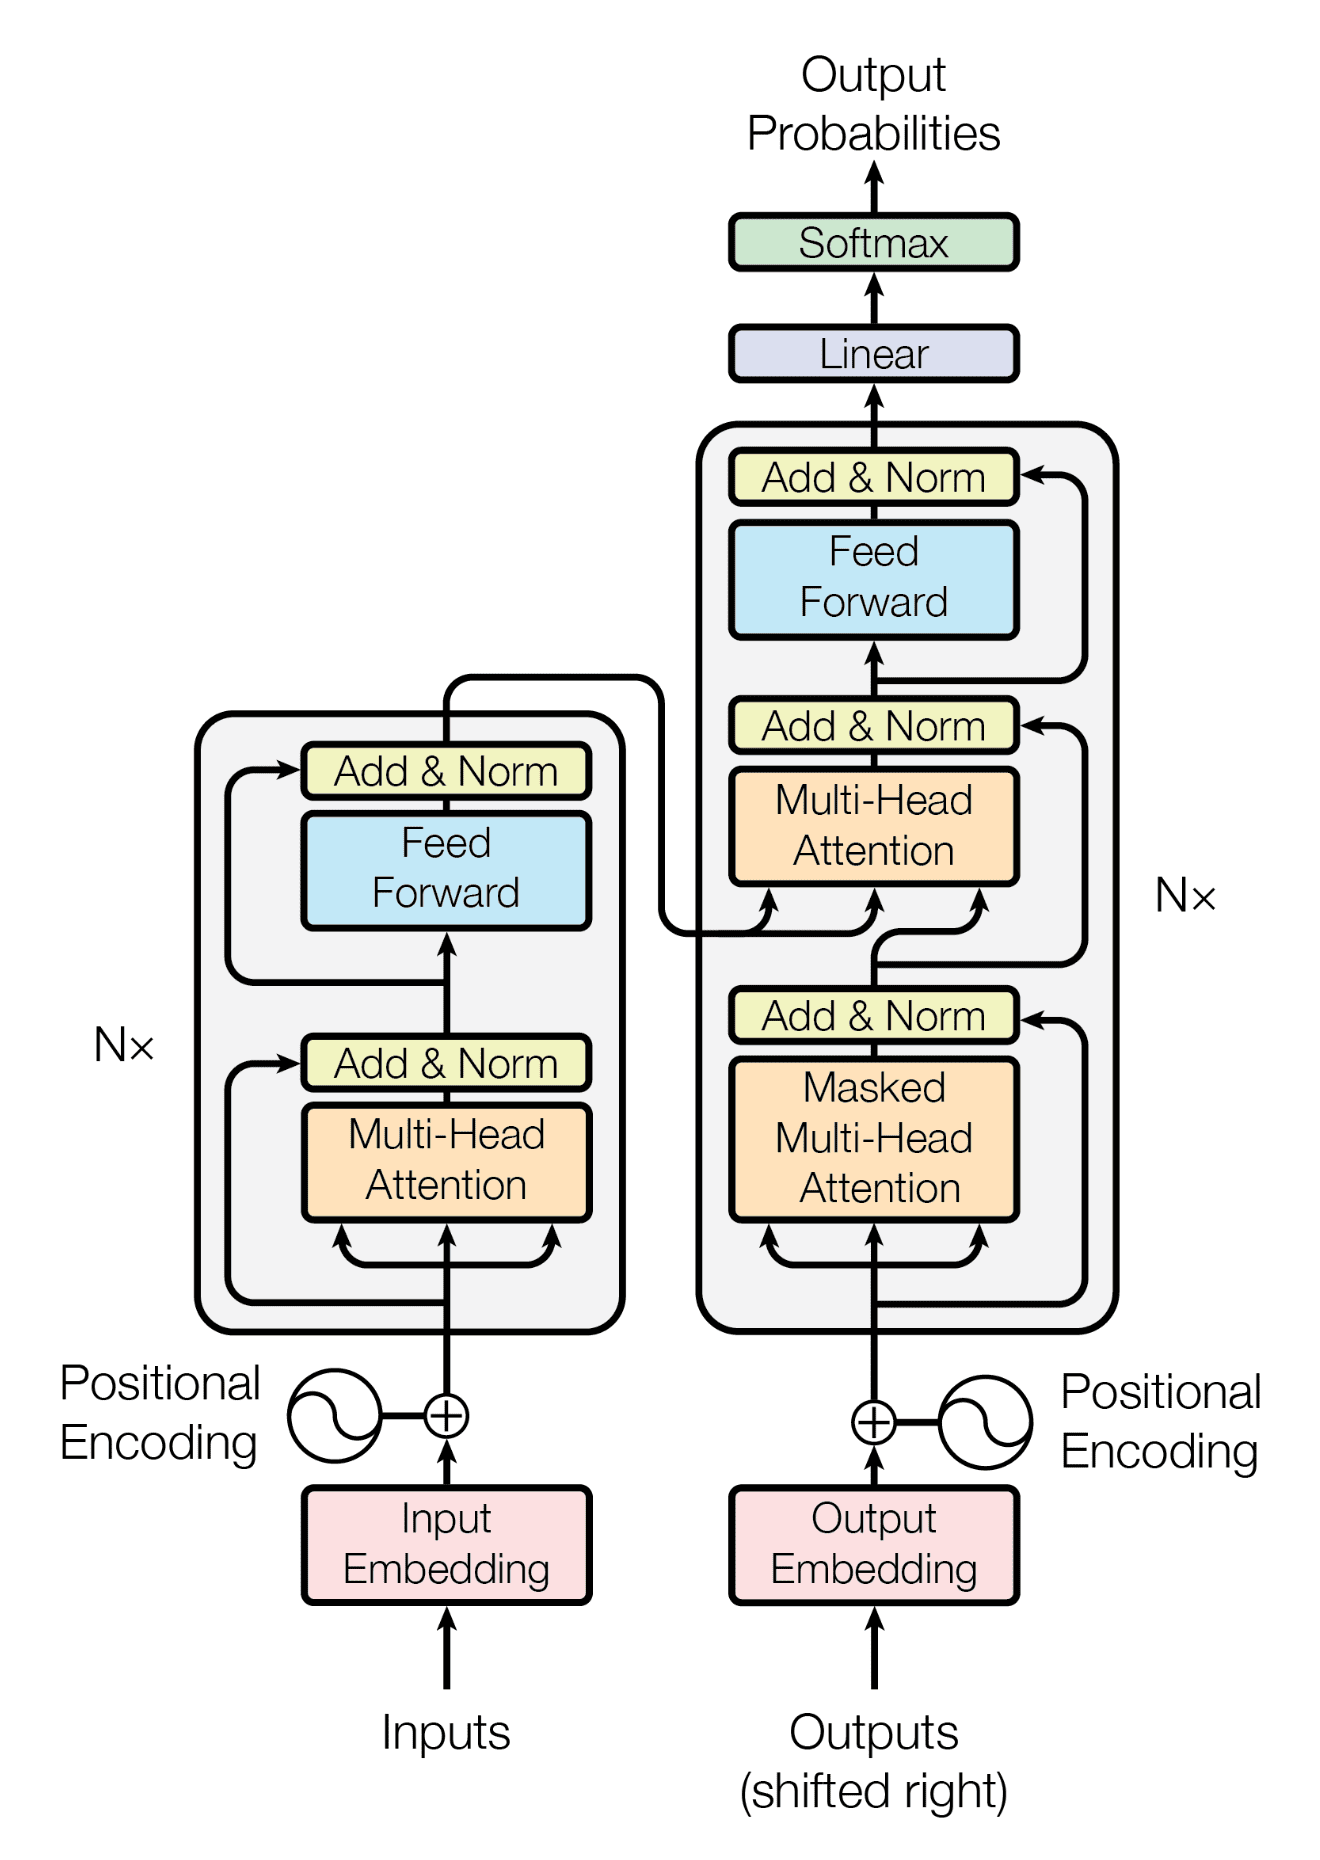
\includegraphics[height=10cm]{attention_research_1.png}
    \label{fig:transformer}
    \caption{Architecture of Transformer\cite{attention}}
\end{figure}

\subsection{Encoder and Decoder}

The architecture of the encoder comprises six homogeneous layers, wherein each layer encompasses two distinct sublayers. The initial sublayer implements a multi-head self-attention mechanism, while the subsequent sublayer employs a positionally entirely connected feed-forward network. Residual connections and layer normalization are put in an application for each sublayer. Consequently, the results of each sublayer are computed as LayerNorm(x + Sublayer(x)), where Sublayer(x) represents the function performed independently by each sublayer. To accommodate these residual connections, all sublayers and embedding layers in the model produce outputs with a dimensionality of $d_{model}$ = 512.

Components of Encoder : 

\begin{enumerate}
   \item Self-Attention Mechanism:
   \begin{enumerate}
        \item Scaled dot-product attention, also known as self-attention, enables the model to selectively centre around particular input sequence chunks. It determines a weighted sum of values (V) by assessing how similar the query (Q), key (K), and value vectors are to one another.
         A number of attention heads are identifiable in each encoder layer, allowing for the capturing of various dependencies and interactions within the sequence.
        
         \item Self-attention uses the Q and K dot product to calculate attention ratings, which are then scaled and normalized using softmax. When calculating the output, these scores are employed to account for the corresponding values.
         \item The encoder effectively captures long-range relationships and accounts for the contextual relevance of each token inside the sequence by using this attention method.


    \end{enumerate}
    
   \item Feed-Forward Neural Network:
    \begin{enumerate}
        \item The output then goes through extra processing through the FFN after the self-attention stage.

        \item A non-linear activation function, similar to ReLU, separates two linear transformations in the FFN.

        \item This network improves the encoder's capacity to detect complex relationships and patterns across distinct sequence segments.


    \end{enumerate}

   \item The Transformer model's architecture includes both layer normalization and residual connections:
    start the enumerationitem The outputs of each sub-layer are normalized using layer normalization after the self-attention mechanism and the feed-forward network.
\begin{enumerate}
        \item Additionally, residual connections are utilized to preserve data from earlier layers and lessen the difficulties associated with the vanishing gradient problem during training.

    \end{enumerate}

    \item Transformers' positional encoding technique is essential for resolving the input sequence's lack of an intrinsic position or order awareness. These techniques are used to accomplish it:


    \begin{enumerate}
      \item  Fixed-length vectors are added to the input embeddings to introduce positional data.
       \item  These vectors' sinusoidal functions of various frequencies give the model the ability to learn about positional relationships while it is being trained.


    \end{enumerate}
\end{enumerate}

The Transformer model's decoder is made up of six identical levels, each with three inferior layers. Self-attention and feed-forward networks are two sub-layers that are similar to the encoder in design. The resultant output derived from the stack of encoders is subjected to multi-head attention by the last small layer, which is exclusive to the decoder. Each sub-layer is enveloped by residual connections in its vicinity. Subsequently, layer normalization is applied. The self-attention sub-layer of the decoder is altered to block access to the following points. The model makes sure that predictions at point 'i' fully depend on known outputs at locations prior to 'i' by including a masking strategy and shifting the output embeddings by one place.



Components of Decoder : 

\begin{enumerate}
   \item The following traits define the decoder's self-attention mechanism:

    \begin{enumerate}
       \item The decoder makes use of self-attention, just like the encoder. It also imposes the restriction that each location in the decoder can only attend to positions that came before it.



      \item To prevent any information from future steps from leaking out during generation, this constraint makes sure that the model only takes leftward positions into account.


        \item The model successfully captures dependencies and relationships between different segments of the generated output sequence by utilizing the self-attention procedure in the decoder.

    \end{enumerate}
    
    \item Encoder-Decoder attention process can be explained as follows:

    \begin{enumerate}
        \item The decoder has an encoder-decoder attention mechanism in addition to self-attention.


       \item The decoder may concentrate on the encoded input sequence produced by the encoder thanks to this method.


      \item This method supports the development of precise and contextually relevant output by matching pertinent parts of the input sequence with the places in the decoder.

    \end{enumerate}

   \item The decoder also incorporates a feed-forward neural network (FFN) to enable further processing:

    \begin{enumerate}
       \item The decoder uses a feed-forward neural network (FFN) for further processing, just like the encoder.
        \item The FFN in the decoder aids in the capturing of intricate interactions and patterns in the output sequence.

    \end{enumerate}

    \item Layer Normalization and Residual Connections:
    \begin{enumerate}
       \item The decoder incorporates a feed-forward neural network (FFN) which is similar to the encoder.
        \item The FFN's inclusion in the decoder makes it easier to detect complex relationships and patterns in the output sequence.

    \end{enumerate}

    \item Positional Encoding:
    \begin{enumerate}
       \item The decoder also builds positional encoding into the model to provide positional information.
        \item The decoder uses sinusoidal functions of various frequencies in the input embeddings to capture positional relationships, just like the encoder does.

    \end{enumerate}
\end{enumerate}

\subsection{Attention function}
A query and a collection of key-value pairs are mapped together to produce an output, which is a brief description of how neural networks' attention function works. These components, including the query, keys, values, and the final result, are all examples of vectors. A weighted sum of the values is computed in order to provide the outcome. A compatibility function that assesses the connection between the query and the relevant key determines the weight assigned to each value. This function's capacity to process attention scores, which measure the significance or importance of distinct points within a sequence, is what gives it its significance. The Transformer model's encoder-decoder attention mechanism and the self-attention mechanism both heavily rely on this attention function. More research will give us a more complex knowledge of how the attention function works.

\begin{figure}[!h]
    \centering
    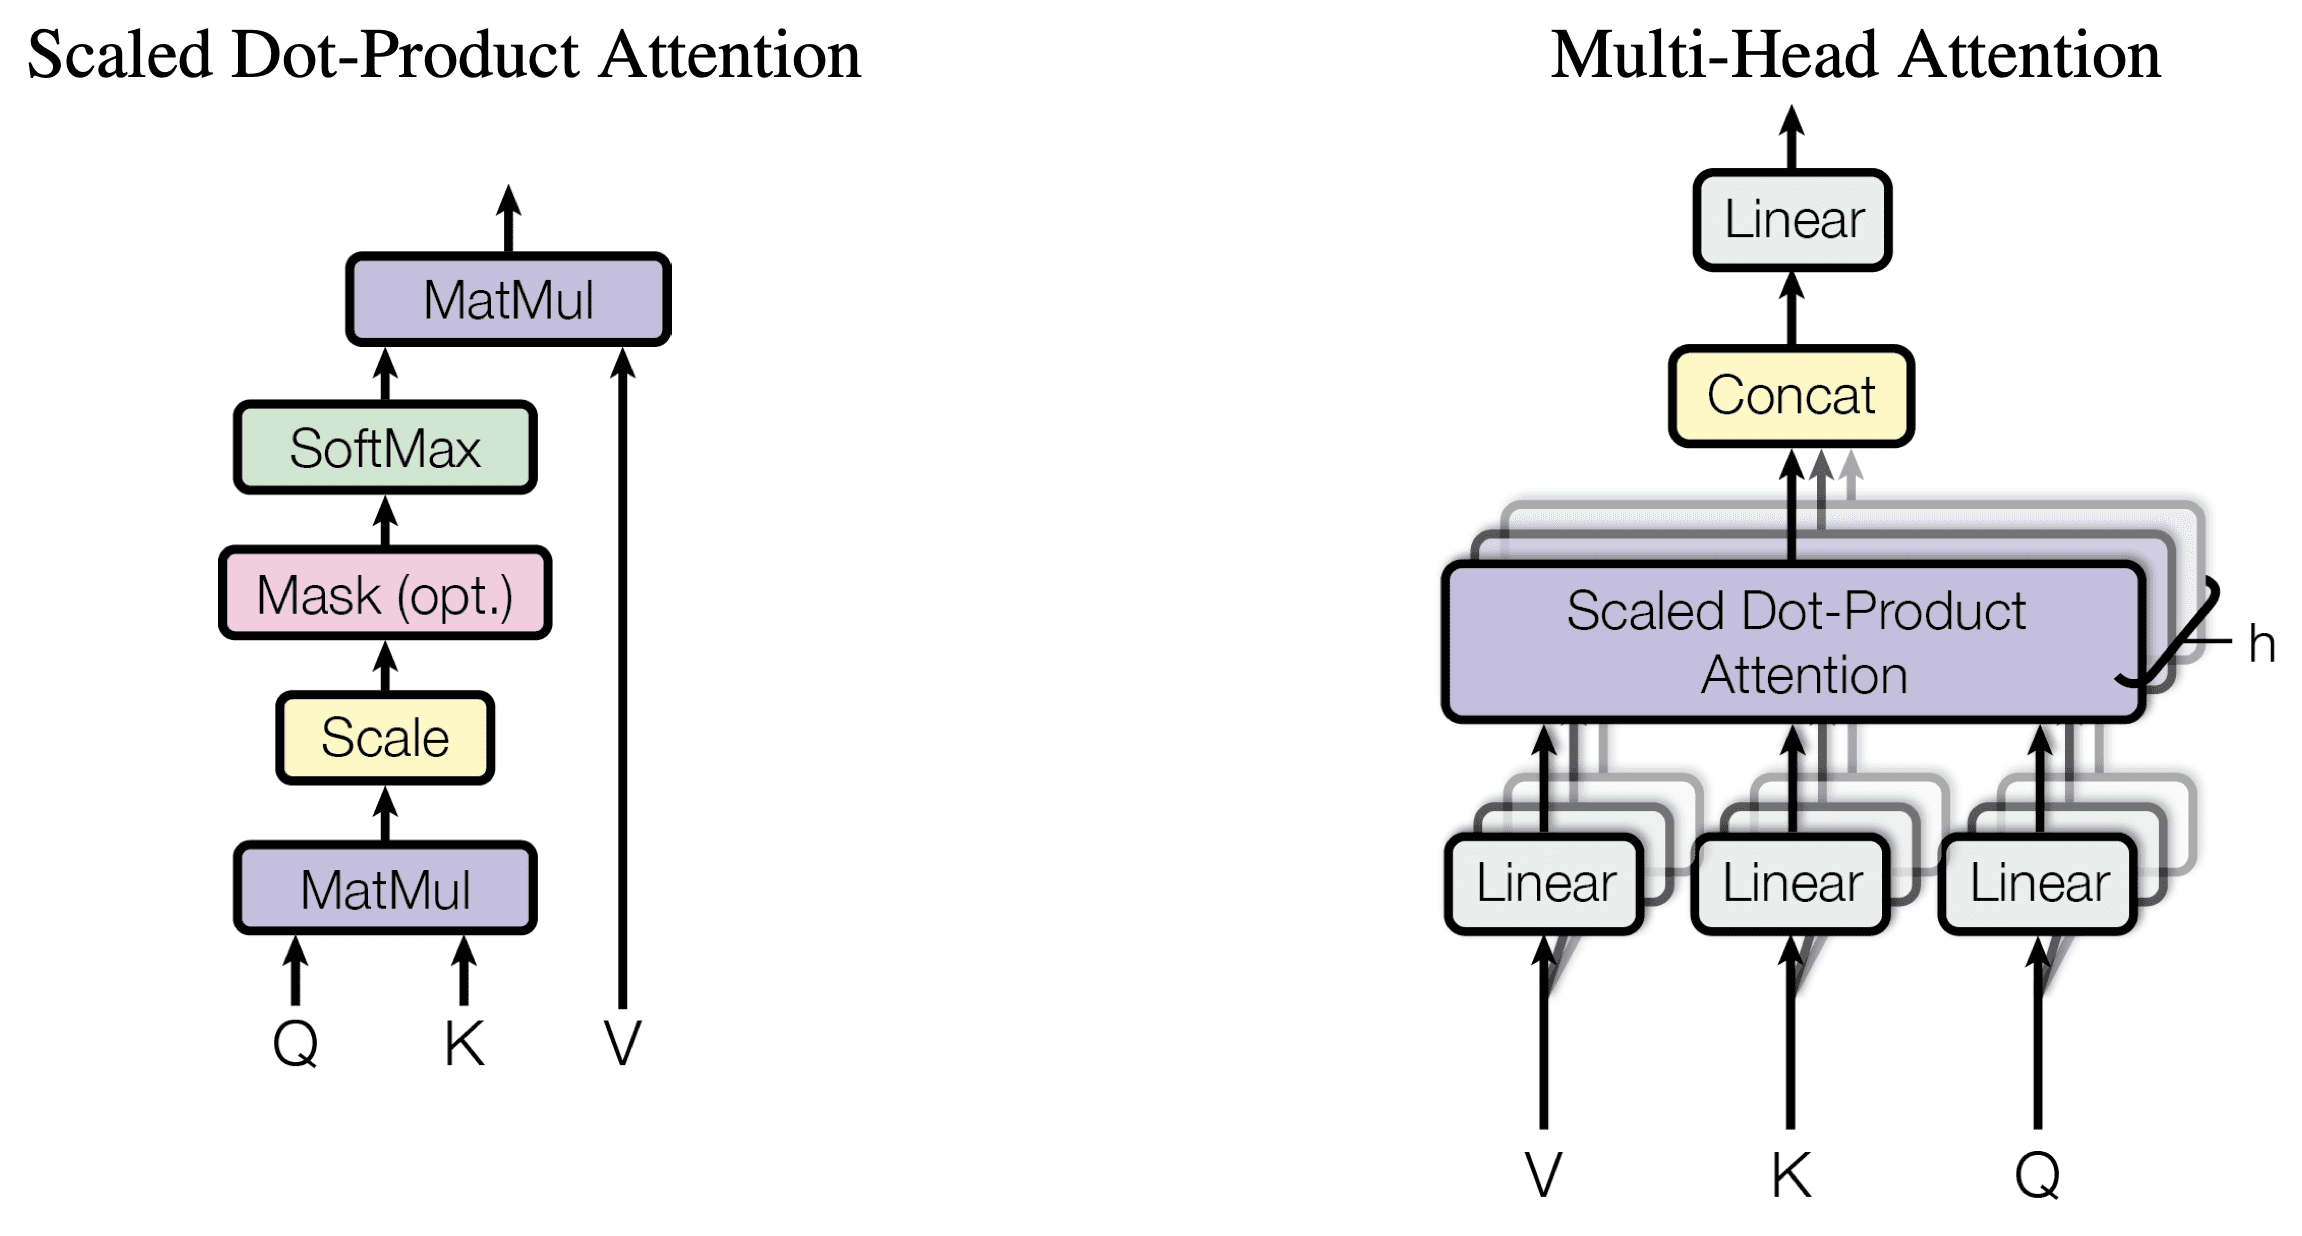
\includegraphics[height=6cm]{dotproduct_1.png}
    \label{fig:dotprod}
    \caption{On the left side, Scaled Dot-Product Attention. On the right side, Multi-Head Attention is depicted, which encompasses multiple attention layers operating concurrently.\cite{attention}}
\end{figure}

As a result, the model may calculate attention scores that reflect the significance or relevance of various points within a sequence. Both the Transformer's encoder-decoder attention mechanism and its self-attention mechanism use the attention function. Let's examine the attention function in greater detail:

\begin{enumerate}
    \item Input Vectors:
    \begin{enumerate}
      \item The three input vectors used by the attention function are : Queries (Q), keys (K), and values (V)
        \item For self-attention and encoder-decoder attention, respectively, these vectors are formed from the output or embeddings of the preceding layer.


    \end{enumerate}

    \item Linear Transformations:
    \begin{enumerate}
      \item The input vectors (Q, K, and V) are linearly transformed using learnt weight matrices before to generating attention ratings.
        \item With the aid of this transformation, the model is able to project the input vectors into a fresh space that more accurately depicts pertinent relationships.


    \end{enumerate}

    \item Dot Product Similarity:
    \begin{enumerate}
         \item The similarity between each key vector (K) and the query vector (Q) is calculated by the attention function using the dot product.
        \item The alignment or agreement of their orientations is measured by the dot product, which then records the similarity between the vectors.


    \end{enumerate}

    \item Scaling:
    \begin{enumerate}
       \item The dot product is adjusted by scaling it with the square root of the dimensionality of the key vectors to prevent big dot products from producing gradients with high magnitudes 
        \item The scaling helps to stabilize the training process and makes sure that the dot products are within a realistic range.


    \end{enumerate}

    \item Attention Scores and Softmax:
    \begin{enumerate}
         \item To determine attention scores, the scaled dot products are run through a softmax function.
        \item The scores are normalized using the softmax function to ensure that they add up to 1 and accurately reflect the relative weight or importance given to each position.


    \end{enumerate}

    \item Weighted Sum of Values:
    \begin{enumerate}
       \item The matching values (V) associated with the key vectors item are weighted using the attention ratings derived from the softmax function. 
      \item The attention function's ultimate result is produced by adding the weighted sum of the values.


    \end{enumerate}

    \item Multiple Attention Heads:
    \begin{enumerate}
        \item The model can pay attention to various patterns or dependencies inside the input sequence thanks to the attention function's many attention heads.
        \item Each attention head produces its own set of attention scores and output and has a unique set of learning weight matrices for linear transformations.


    \end{enumerate}
\end{enumerate}

By giving distinct places varied degrees of importance, the attention function allows the Transformer model to capture dependencies and relationships within a sequence. The Transformer can efficiently model long-range dependencies and produce contextually informed representations during both training and inference by incorporating self-attention and encoder-decoder attention methods.

% \subsubsection{Scaled Dot-Product Attention}

% The attention mechanism employed in our study is denoted as "Scaled Dot-Product Attention" (Figure \ref{fig:dotprod}). The input to this attention mechanism consists of queries, keys with a dimensionality of $d_k$, and values with a dimensionality of $d_v$. To calculate the weights assigned to the values, we perform dot products between the query and each key, scale them by a factor of $\sqrt{d_k}$, and then apply the softmax algorithm.

% In practice, the attention function is computed simultaneously for a set of queries that are organized into a matrix Q. Similarly, the keys and values are combined into matrices K and V, respectively. The output matrix is determined using the following calculation:

% \begin{center}
%     $
%     Attention(Q, K, V) = softmax(\frac{QK^T}{\sqrt{d_k}})V
%     $
% \end{center}

% Additive attention and dot-product (multiplicative) attention are the two most often employed attentional functions. The only difference between dot-product attention and our technique is the scaling factor, which is $\frac{1}{\sqrt{d_k}}$. The compatibility function is computed using additive attention, employing a feed-forward network with a single hidden layer. While both methods are theoretically equivalent in terms of complexity, in practice, dot-product attention proves to be faster and more space-efficient. This is due to its ability to leverage highly optimized matrix multiplication code for implementation.

% For bigger values of $d_k$, additive attention outperforms dot product attention without scaling, although the two processes perform comparably for small values of $d_k$. We postulate that as the dimensionality ($d_k$) of the query and key vectors increases, the magnitudes of the dot products also grow, thereby compelling the softmax function towards regions characterized by very small gradients\footnote{Consider the assumption that the components of $q$ and $k$ are independent random variables with a mean of 0 and a variance of 1. This assumption aids in illustrating the reason behind the magnification of dot products. Consequently, their dot product, $q \cdot k = \sum_{i=1}^{d_k} q_ik_i$, has an average value of 0 and a variance of $d_k$.}. To counterbalance this effect, we scale the dot products by $\frac{1}{\sqrt{d_k}}$.


% \subsubsection{Multi-Head Attention}

% We discovered that linearly projecting the queries, keys, and values with separate learned linear projections to dimensions $d_k$, $d_k$, and $d_v$ respectively, proved to be advantageous compared to employing a single attention function with $d_{model}$-dimensional keys, values, and queries. Consequently, the attention function is applied concurrently to each of the projected versions of queries, keys, and values, resulting in output values of dimension $d_v$. These output values are subsequently concatenated and projected once again, as illustrated in Figure \ref{fig:dotprod}.


% The utilization of multi-head attention in the model enables the simultaneous attention to be directed towards multiple representation subspaces at different positions. This capability allows for the joint consideration of diverse sets of data. In contrast, when employing a single attention head, the averaging process inhibits the model's ability to jointly attend to data across different representation subspaces and positions.

% \begin{center}

%     MultiHead($Q, K, V$) = Concat($head_1, ..., head_h$)$W^{O}$
    
%     where $head_i$ = Attention($QW_i^{Q}, KW_i^{K}, VW_i^{V}$)

% \end{center}

% The projections in this context refer to matrices $W_i^{Q} \in \mathbb{R}^{
% d_{model}×d_k}$, $W_i^{K} \in \mathbb{R}^{
% d_{model}×d_k}$, $W_i^{V} \in \mathbb{R}^{
% d_{model}×d_v}$.

% In this study, we employ a configuration consisting of $h$ = 8 parallel attention layers, commonly referred to as heads. For each attention head, we set the dimensions of the keys ($d_k$) and values ($d_v$) as $d_{model}/h$ = 64. This choice is made to ensure a comparable overall computing cost to that of single-head attention with the full dimensionality, despite the reduced dimensionality in each individual head.


% \subsection{Applications of Attention in a Transformer}

% \begin{itemize}
%     \item In "encoder-decoder attention" layers, memory keys and values are derived from the encoder's output, while queries are obtained from the preceding decoder layer. Consequently, the decoder can undertake the position in the input sequence.
%     \item The encoder incorporates self-attention layers. All of the keys, values, and queries in a self-attention layer are derived from the same source, in this instance the encoder's output from the layer below. Each position within the encoder has access to all positions in the stratum beneath it.
%    \item Similar to this, the self-attention layers of the decoder allow each position to pay attention to all positions preceding it. To preserve the decoder's auto-regressive property, we must prohibit leftward information flow. We implement this within scaled dot-product attention by masking (setting to) all input values of the softmax that correspond to unauthorized links.



 
% \end{itemize}

% \subsection{Why Self-attention}
%  We are going to compare various features of the self-attention layers to the recurrent and convolutional layers regularly utilized for mapping one variable-length sequence of symbol representations
% ($x_1, ..., x_n$) to another sequence of equal length ($z_1, ..., z_n$), with $x_i, z_i \in \mathbb{R}^d$, such as a hidden
% layer in a typical sequence transduction encoder or decoder. Motivating our usage of self-attention we
% can consider three desiderata.

% One is the aggregate computational complexity of every layer. The amount of computation ehich can be parallelized is set by the minimum number of sequential operations required.


% The third area of interest is the examination of long-distance dependencies within a network. Several sequence transduction activities are significantly hampered by the acquisition of long-range dependence. The distance that signals must travel in both forward and reverse directions has an impact on the network's ability to understand these dependencies. The learning of long-range dependencies is made easier by the short distances that these routes have between any two points in the input and output sequences. As a result, among networks made up of various layer types, a comparison of the maximum path length between any two points in the input and output sequences is made.

\section{BERT}

Google AI Language researchers recently published a paper titled "Bidirectional Encoder Representations from Transformers"(BERT \cite{BERT}). It resulted in heated conversations and debates in the machine learning field by revealing novel discoveries in a broad range of NLP tasks. These include Question Answering and Natural Language Inference among others.

BERT contributed significantly to language modelling by employing bidirectional training of the Transformer, a notable model employing attention mechanisms. Previous approaches differ from this one by processing text sequences in a left-to-right order or by combining left-to-right and right-to-left orientations in training. Initial findings indicate that a language model trained in two orientations has a greater understanding of linguistic context and flow than its counterparts trained in a single direction. The researchers introduce the Masked Language Model (MLM), a ground-breaking strategy that pioneers bidirectional training in models where such an approach was previously impractical.





\subsection{Background}

Transfer learning in computer vision entails preparatory training of a neural network model on a well-known task, and refining it afterwards to serve as the base to be constructed for a new model with a specific purpose. Recent research has shown that a kindred approach can be useful for a wide array of natural language tasks.

A distinct approach is feature-based training, prevalent in NLP applications and illustrated in the most recent ELMo publication. A pre-trained neural network is used to generate word embeddings, subsequently utilized as features in NLP models.



\subsection{Explaining BERT}

BERT is a sophisticated language model designed to enhance the complexity of machine learning and the understanding of linguistic context. It was initially developed by Google and has since evolved into a potent NLP tool.

BERT's foundation is the Transformer architecture and functions as a mechanism that can comprehend contextualized relationships related to words and their subcategories in various situations and contexts. A typical Transformer is comprised of a decoder that produces a prediction and an encoder that scans the input text. However, BERT only employs the encoder mechanism, which is consistent with its objective of developing a language model.


In contrast to standard models, which read text word by word, the Transformer encoder utilized by BERT scans the whole sequence of terms simultaneously. This allows it to comprehend a word's contextual behaviour in regard to the entirety of its surroundings, effectively rendering it bidirectional. However, nondirectional would be a better term because it does not inherently favour any particular direction.
A series of tokens (words or subwords) are implanted into vectors by the Transformer encoder prior to neural network processing. The product consists of a series of H-dimensional vectors, each correlated with a token with the same index as the input.

It is challenging to determine a forecasted objective at the time of language model training. Numerous models forecast the following term in a sequence. However, this strategy restricts context-based learning opportunities. BERT employs two distinct training techniques to surmount this challenge.

\begin{figure}[!h]
    \centering
    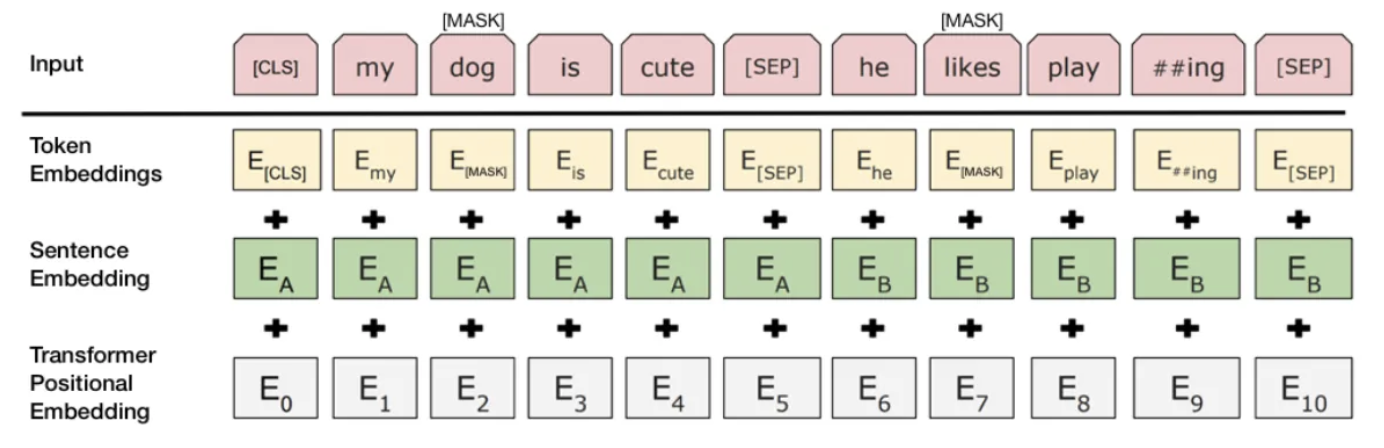
\includegraphics[width=0.7\textwidth]{images/nsp.png}
    \label{fig:nsp}
    \caption{Input representation for BERT\cite{BERT}}
\end{figure}


The first of these techniques involves the pre-training of deep bidirectional depictions of unassigned wording. This is accomplished through the use of joint conditioning on the left and right contexts across all layers. Consequently, state-of-the-art models for a variety of tasks can be created by incorporating a single output layer into the preliminary trained BERT model. These activities, such as language inference and query answering, do not necessitate significant architectural modifications.

BERT uses masked language modelling as a strategy to enhance instruction. In this method, a portion of the input tokens are unsystematically muted, and the model is then instructed to determine the original vocabulary id of the muted word depending on the circumstances. This technique authorizes the model to understand not only the connotation of the words but also their relationships within a phrase.

\begin{figure}[!h]
    \centering
    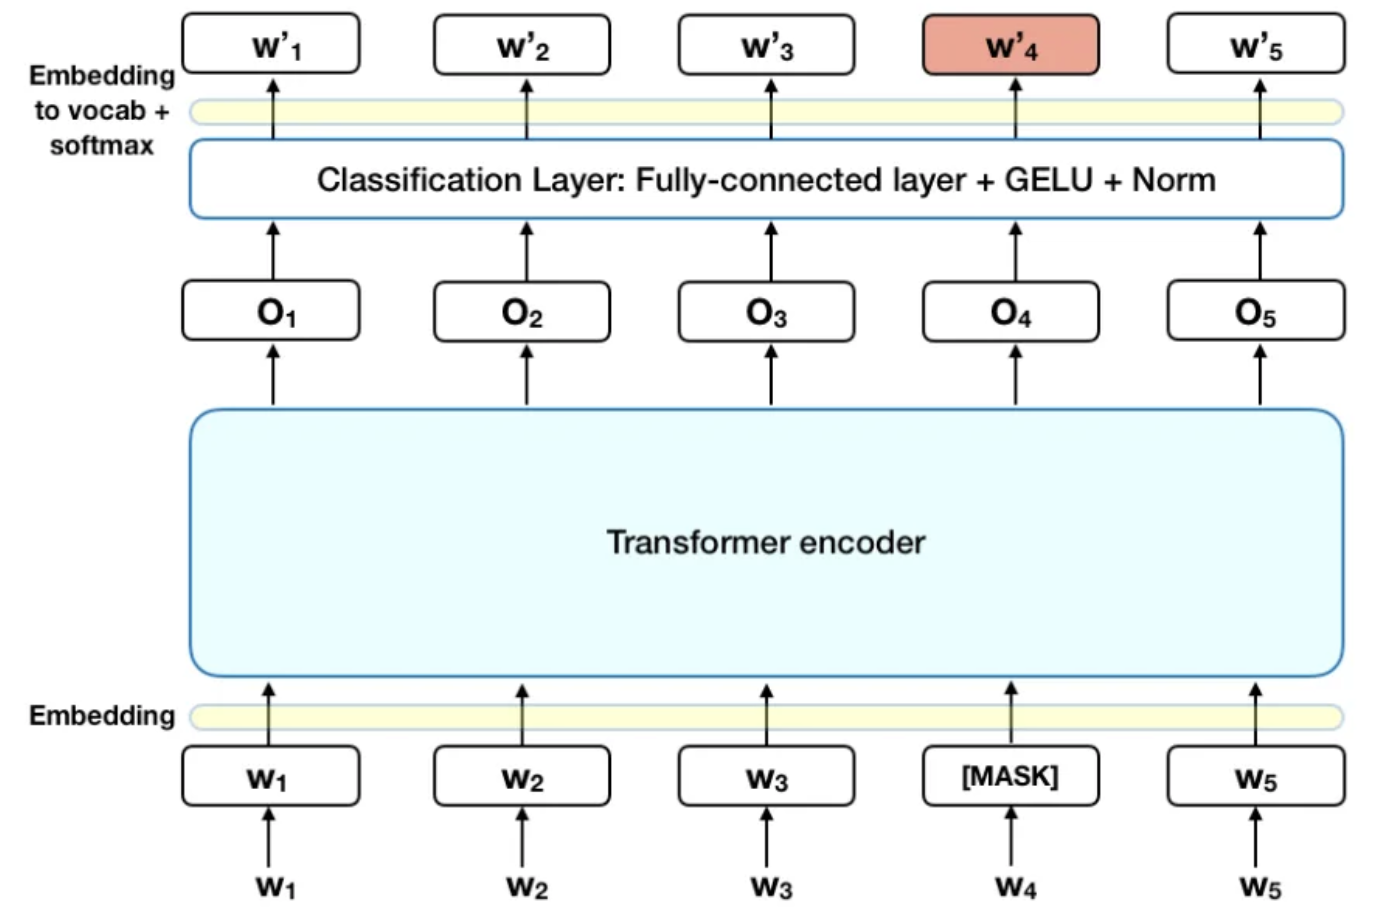
\includegraphics[width=0.7\textwidth]{images/mlm.png}
    \label{fig:mlm}
    \caption{BERT functioning mechanism breakdown\cite{towardsdatascience}}
\end{figure}



Due to its context-centred approach and non-directional nature, BERT provides a reliable method for language modelling. It is a powerful tool in the disciplines of AI and machine learning due to its pre-training and fine-tuning procedures, which allow it to execute exceptionally well on diverse NLP jobs. It has proven to be both theoretically simple and practically effective, allowing for further language processing research and development.

The diagram depicts the operational workflow of the Transformer encoder. As system inputs, a collection of tokens initially transformed into vector embeddings serve. The neural network is then applied to these embedded vectors for processing. The final output of the system is a collection of H-dimensional vectors. Each output vector corresponds to an input token with the same index, and the output vectors are aligned with the input tokens.



In the field of language model training, defining a prediction objective is extremely complex. In numerous models, the method of predicting the next word in a series has been incorporated. However, this unidirectional method inherently restricts context-based learning. BERT employs two distinct training methods to mitigate the effects of these restrictions.





% \subsubsection{Masked LM (MLM)}

% Before feeding word sequences into the BERT, 15\% of each sequence's words are modified with a [MASK] token. Using the context provided by the non-masked words in the sequence, the model then attempts to predict the original value of the masked words. Technically, the output word prediction necessitates:





% \begin{itemize}
%      \item On top of the encoder output, a classification layer is added, and the output vectors are multiplied by the embedding matrix to generate the vocabulary dimension.
%      \item Determine the probability of each word in the lexicon using softmax.




% \end{itemize}

% \begin{figure}[!h]
%     \centering
%     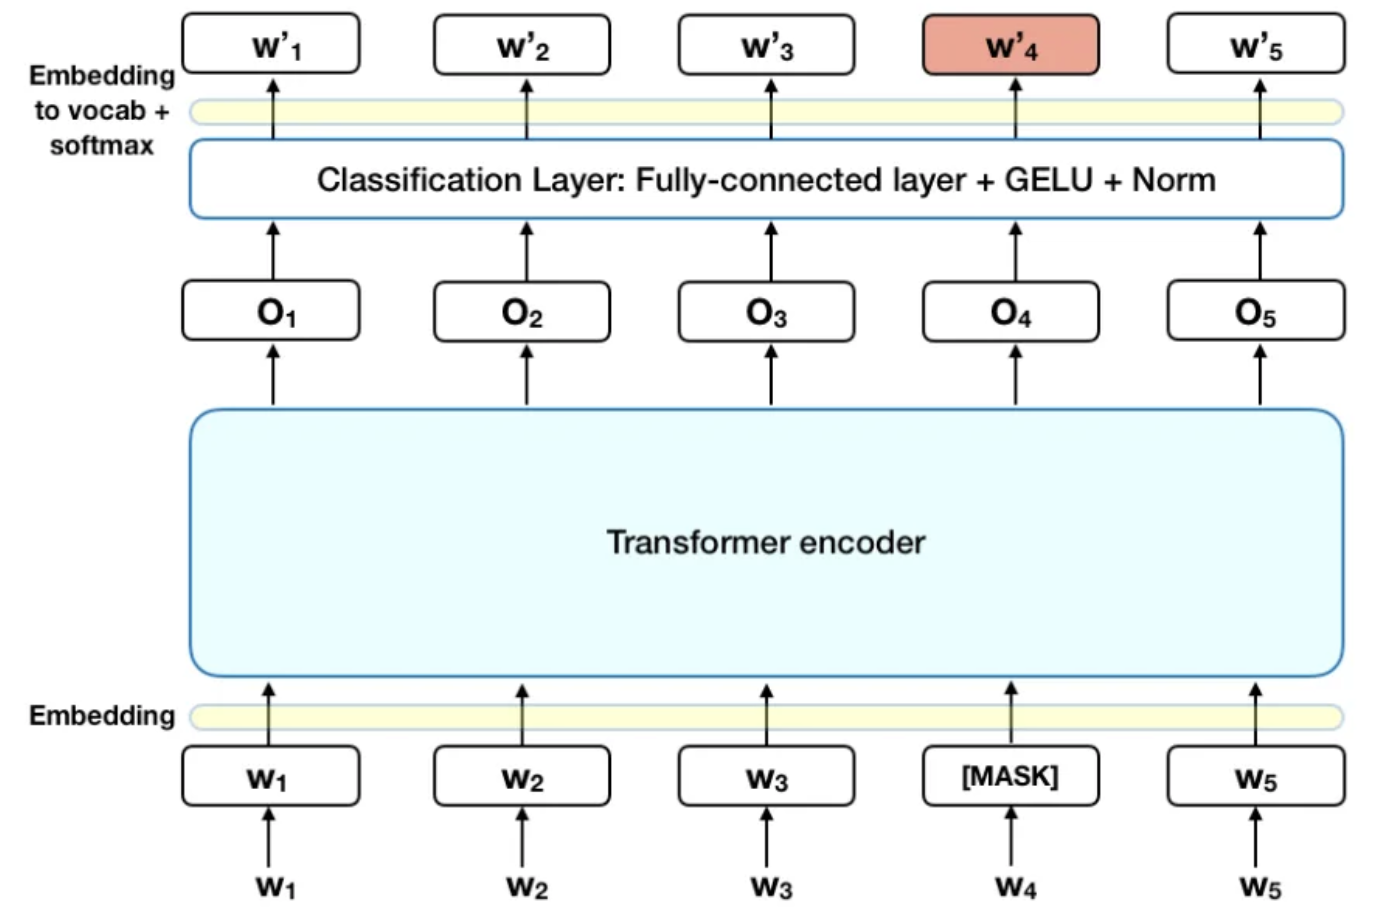
\includegraphics[width=0.7\textwidth]{images/mlm.png}
%     \label{fig:mlm}
%     \caption{NLP State-of-the-art language model}
% \end{figure}

% The BERT loss function disregards the prediction of non-masked terms and only considers the prediction of masked values. Compared to directional models, the model's delayed convergence rate is compensated for by its enhanced context awareness.



% \subsubsection{Next Sentence Prediction (NSP)}

% As the Bidirectional Encoder Representations from Transformers (BERT) model is being trained, it is supplied pairs of sentences. The primary objective is to equip the model with the ability to determine whether the second sentence of a pair follows the first in the original text. Half of the examples in the training process consist of pairings in which the second sentence follows the first in the original context, while the other half consist of pairs in which the second sentence is randomly selected from the corpus. It is anticipated that the sentence selected at random will lack cohesion with the previous sentence. During the training phase, the input is processed prior to being fed to the model so that it can distinguish between the two sentences that comprise the combination.







% \begin{itemize}
%     \item The first sentence begins with a [CLS] token, and each subsequent sentence ends with a [SEP] token.
%     \item Each token contains an embedded sentence that identifies either Sentence A or Sentence B. Sentence embeddings and token embeddings with a vocabulary of 2 share a similar concept.
%     \item Each token is assigned a positional embedding to indicate its position within the sequence. This paper describes the theory and practice of positional embedding.

% \end{itemize}


% \begin{figure}[!h]
%     \centering
%     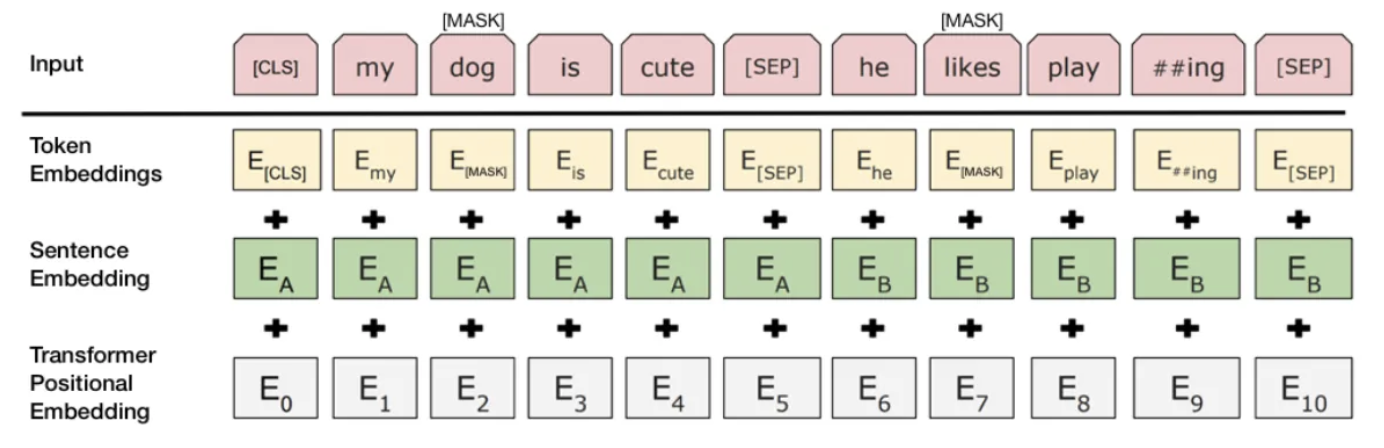
\includegraphics[width=0.7\textwidth]{images/nsp.png}
%     \label{fig:nsp}
%     \caption{Input representation for BERT}
% \end{figure}

% The following steps are performed to determine whether the second statement is in fact related to the first.




% \begin{itemize}
%     \item The entire input sequence goes through the Transformer model.
%     \item The output of the [CLS] token is altered into a 2×1 shaped vector, with the help of a simple classification layer (learned matrices of weights and biases).
%     \item The usage of softmax in order to calculate the likelihood of IsNexSequence.
% \end{itemize}

% When training the BERT model, Masked LM and Next Sentence Prediction are simultaneously learnt in order to minimize the merged loss function of our two techniques.


\subsection{Usage of BERT (Fine-tuning)}

The BERT paradigm can be easily applied to certain jobs and does not necessitate significant changes to the fundamental model. Fine-tuning is a technique that can be put into application to a variety of linguistic tasks with little modification to the fundamental model.

A classification layer is added to the Transformer yield for the [CLS] token for classification tasks like sentiment analysis, simulating the Next Sentence classification process. Due to its aptitude for comprehending context and semantic relationships, BERT is now able to solve text categorization problems using a similar architecture.


When it comes to Question Answering Tasks, BERT is tasked with finding the answer inside a given written succession after being given a question in regards to it. The model is effectively instructed to perform Question Answering tasks by teaching it two additional vectors that specify the beginning and conclusion of the answer.

For NER, BERT is given a text sequence and instructed to identify different kinds of entities (such as Person, Organization, Date, etc.) that are contained in the written work. The model is able to correctly detect and categorize various items within the text because it has been instructed by feeding the output vector of every token to a layer used for classification purposes that forecasts the labelling of NER.



Between the initial BERT practice and the fine-tuning procedure, the majority of hyper-parameters remain stable. The original BERT publication, however, offers detailed instructions on the hyper-parameters which might necessitate adjusting throughout this procedure. The BERT team has been successful in obtaining cutting-edge results using these fine-tuning methods on a wide spectrum of difficult natural language tasks.

% \subsection{Takeaways}

% Even at very large sizes, a model's size has a major impact on how well it performs. The comparison of BERT\_large and BERT\_base makes this idea very evident. The more comprehensive model of its kind is the former, which has 345 million parameters. In tasks carried out on a smaller scale, empirical evidence has demonstrated a definite advantage over the BERT basic model. The latter has the same architecture but has 110 million fewer parameters than the former.


% Given enough training data, the connection between the number of training steps and model accuracy shows that increasing the number of training steps often results in an increase in model accuracy. This fact is particularly clear in the MNLI problem, where training the BERT\_base model with 1 million steps (with a batch size of 128,000 words) results in a 1.0 \% gain in accuracy compared to training it with 500,000 steps while maintaining the batch size constant.

% Due to the fact that only 15\% of words are predicted in each batch, the Masked Language Model (MLM), the bidirectional training method used by BERT, converges more slowly than traditional left-to-right methods. After a limited number of pre-training stages, the bidirectional training methodology still outperforms left-to-right training despite its slower convergence. These details emphasize how creative BERT's method for handling jobs involving natural language processing is.

% \begin{figure}[!h]
%     \centering
%     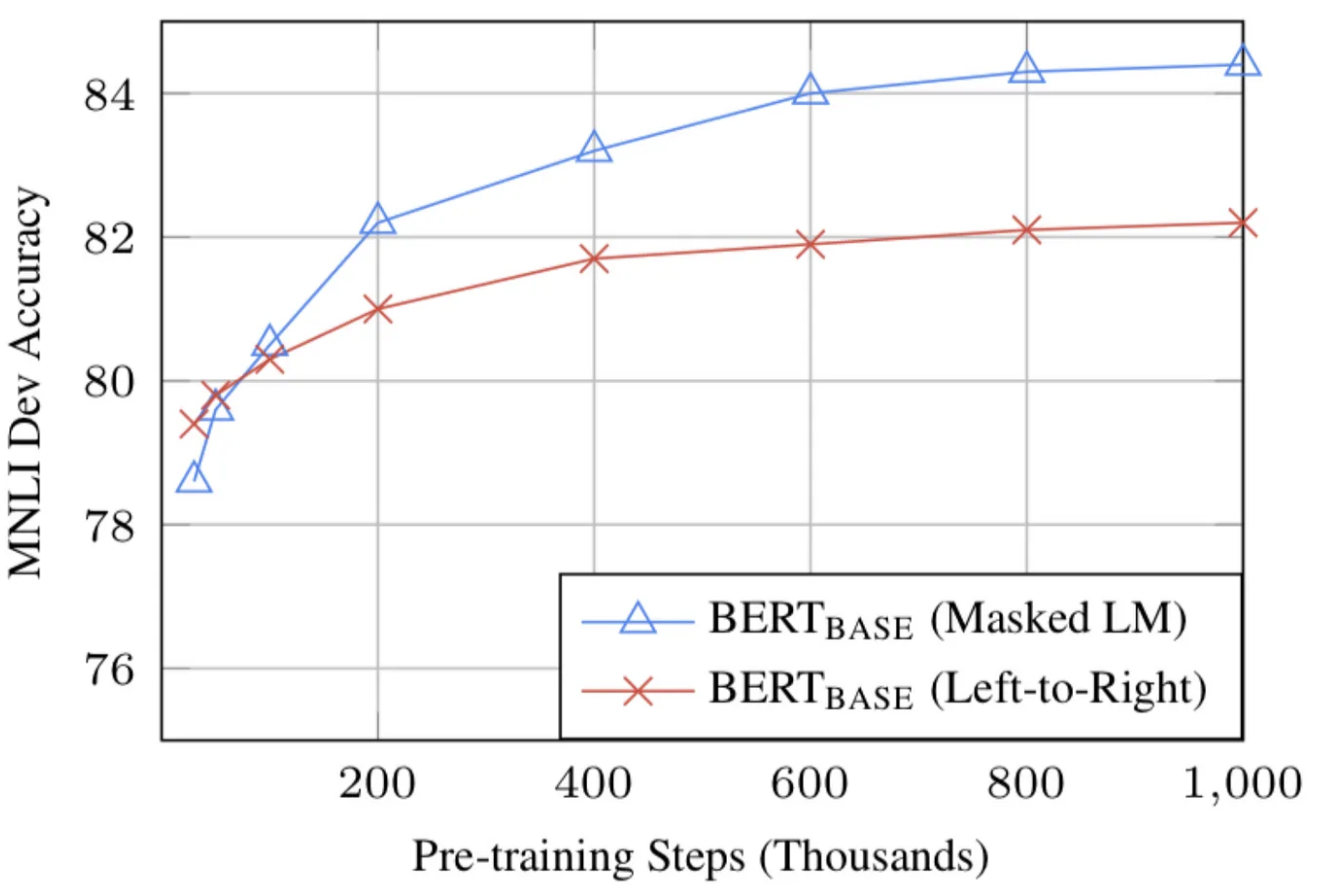
\includegraphics[width=0.7\textwidth]{images/takeaways.png}
%     \label{fig:takeaways}
%     \caption{My caption}
% \end{figure}

\section{Hugging Face}

Hugging Face\footnote{https://huggingface.co/} is primarily an open-source platform and library created exclusively for NLP jobs. Its goal is to democratize AI by giving academics and developers easy-to-use tools. Hugging Face has developed a thriving and welcoming community that encourages cooperation and knowledge exchange among NLP fans throughout the world.

\subsection{Features and Benefits}
Hugging Face is a valuable tool for NLP practitioners thanks to its many features and advantages. The enormous selection of pre-trained models, which includes the highly regarded BERT model, is one of its standout features. Hugging Face's Model Hub makes these models easily accessible, allowing transfer learning and hastening the creation of NLP applications.



The transformers library from Hugging Face also acts as a complete toolkit for creating, honing, and deploying NLP models. With a large number of utilities and abstractions available to developers, this library streamlines the entire model development life cycle. Pipelines, which are high-level APIs for typical NLP tasks like written content categorization and named entity recallection, are also included in the library, making it simple to create complex NLP systems.

Additionally, Hugging Face emphasizes teamwork and model sharing heavily. Its user-friendly platform allows academics and developers to share their models, building an ecosystem that is driven by the community and advantageous to all parties. The advancement of NLP is made possible by this collaborative atmosphere, which encourages the sharing of ideas, best practices, and novel strategies.



\subsection{Hugging Face's Integration of BERT}

Hugging Face was essential in getting BERT well-known and available to the NLP community. Hugging Face offers pre-trained BERT models through its Model Hub, allowing developers and researchers to take advantage of BERT's capability without the requirement for time-consuming training. Hugging Face's transformers library also provides seamless connection with BERT, enabling users to quickly and easily modify the model for particular NLP needs.

